\documentclass[12pt,a4paper]{article}
\usepackage{mathtools}
\usepackage{parskip}
\usepackage[colorlinks=true, urlcolor=blue]{hyperref}
\usepackage{amsmath}
\usepackage{amssymb}
\usepackage{float}
\usepackage{fontenc}
\usepackage{graphicx}
\usepackage{caption}
\usepackage{subcaption}
\usepackage{multirow}

\renewcommand\thesubsection{\thesection.\arabic{subsection}}
\renewcommand\thesubsubsection{\thesubsection.\alph{subsubsection}}

\newcommand{\tab}{\hspace*{2em}}

\title{ADNI Progress report}
\author{Devendra Goyal\\Uniqname: devendra}

\date{\today}

\begin{document}
\maketitle

\part{Using HMMs to predict disease progression}

\section{Statistics about the data}
\label{sec:data}

There are several choices here for the dataset to be used:

\begin{itemize}
\item One of MRI/PET/CSF only
\item Some combination of 2/3 available modalities
\item Use all three modalities
\item Add demographics data to any of the above options
\end{itemize}

\emph{For now}, I have decided to use only the FDG-PET data for the
HMM problem. 

The pros are:

\begin{itemize}
\item The PET data is the cleanest and most easy dataset to process.
\item The feature space is relatively low dimensional. It is
  the \[mean, median, mode, min, max, stdev\] of the glucose
  expression for 5 expert defined regions in the brain - making it a
  total of 30 features for each patient.
\item Don't have to deal with failed segmentation amongst patients, or
  missing variables. This dataset was processed by the latest
  available package in the field, and the lab releasing it has cleaned
  it perfectly for plug-and-play use.
\item The pre-processing for PET scans accross all ADNI cohorts
  (ADNI1, ADNIGO, ADNI2) was done in one go by the same group using
  the same software, guaranteeing us homogenity in the data.
\end{itemize}

The cons are:

\begin{itemize}
\item Throwing away a lot of useful information from MRIs, CSFs, demographics
\item A small number of patients ($=720$) have more than one PET scan
  (accross all cohorts), which
  could making learning the HMM a problem
\end{itemize}

Some possible solutions for the future:

\begin{itemize}
\item It is potentially a very interesting problem to think about the
  use of observations from multiple modalities in a HMM setting. The
  reason this is better than doing it in an SVM setting is - due to
  the generative nature of the HMMs, we do not have to throw away
  patients who have missing observations for any of the three modalities.
\item For the same reason as above, it will be interesting to think
  about the problem of dealing with missing data.
\end{itemize}

There are a total of 1404 patients accross all three cohorts
with PET data, out of which only 1398 have baseline diagnoses. Out of
those, only \textbf{720 patients} have more than one visit. The
distribution for these patients is as follows:

\begin{tabular}[H]{c | c | c | c | c | c}
  & NL & \multicolumn{3}{|c|}{MCI} & AD\\
\hline
& & MCI-c & MCI-nc & MCI-rev &\\
\hline
FDG-PET & 225 & 126 & 237 & 30 & 102\\
\end{tabular}

\begin{figure}[H]
  \centering
  \includegraphics[width=\textwidth]{pet-dx-visits.png}
  \caption{Diagnoses of patients who had usable PET scans}
\end{figure}

\begin{figure}[H]
  \centering
  \includegraphics[width=\textwidth]{pet-mean.png}
  \caption{Histograms of the MEAN of FDG scans for different diagnoses}
\end{figure}
\begin{figure}[H]
  \centering
  \includegraphics[width=\textwidth]{pet-median.png}
  \caption{Histograms of the MEDIAN of FDG scans for different diagnoses}
\end{figure}
\begin{figure}[H]
  \centering
  \includegraphics[width=\textwidth]{pet-mode.png}
  \caption{Histograms of the MODE of FDG scans for different diagnoses}
\end{figure}
\begin{figure}[H]
  \centering
  \includegraphics[width=\textwidth]{pet-min.png}
  \caption{Histograms of the MIN of FDG scans for different diagnoses}
\end{figure}
\begin{figure}[H]
  \centering
  \includegraphics[width=\textwidth]{pet-max.png}
  \caption{Histograms of the MAX of FDG scans for different diagnoses}
\end{figure}
\begin{figure}[H]
  \centering
  \includegraphics[width=\textwidth]{pet-stdev.png}
  \caption{Histograms of the STDEV of FDG scans for different diagnoses}
\end{figure}

Shown below are histograms to depict the distribution of patients
having varying number of visits. Note that for cases where the
histogram shows patients having data from two different sources, only
cases where the data occurs from the \textbf{same visit} is
considered.

\begin{figure}[H]
  \centering
  \includegraphics[width=\textwidth]{pet-visits.png}
  \caption{Distribution of patients who had PET scans}
\end{figure}
\begin{figure}[H]
  \includegraphics[width=\textwidth]{mri-visits.png}
  \caption{Distribution of patients who had MRI scans}
\end{figure}
\begin{figure}[H]
  \centering
  \includegraphics[width=\textwidth]{csf-visits.png}
  \caption{Distribution of patients who had CSF data}
\end{figure}
\begin{figure}[H]
  \includegraphics[width=\textwidth]{mri-pet-visits.png}
  \caption{Distribution of patients who had MRI+PET scans}
\end{figure}
\begin{figure}[H]
  \centering
  \includegraphics[width=\textwidth]{pet-csf-visits.png}
  \caption{Distribution of patients who had PET+CSF data}
\end{figure}
\begin{figure}[H]
  \includegraphics[width=\textwidth]{mri-csf-visits.png}
  \caption{Distribution of patients who had MRI+CSF data}
\end{figure}
\begin{figure}[H]
  \includegraphics[width=\textwidth]{mri-pet-csf-visits.png}
  \caption{Distribution of patients who had MRI+PET+CSF data}
\end{figure}

\part{Establishing the baseline}

\section{Statistics about the Data}
\label{sec:stats}

The results shown in this document are based on the ADNI-1
cohort. There are several pros and cons of this decision:

\subsection{Pros}

\begin{itemize}
\item All the pre-processed features uploaded on the ADNI website
  operate on the entire cohort, thus there is homogeneity in terms of
  the features available for each patient across each modailty. MRI
  images for ADNI-GO/2 have been processed using different versions of
  the same software, and are also collected using a higher resolution
  MRI machine. While this is not a dealbreaker per se, it will require
  significantly more work to process all the images using the same
  software and generate similar features.
\item Most of the recent literature (~5 years) relies on data from ADNI1
  only to report results. This will give us a chance to compare our
  results directly with some of these reported results.
\item ADNI-1 is the best dataset to track patients longitudinally, as
  it was started in $2004$ and we have about $8$ years' worth of data
  for all MCI and AD patients that the protocol chose to follow (more
  on this later). 
\end{itemize}

\subsection{Cons}

\begin{itemize}
\item ADNI1 has CSF data available for only about 20\% of the
  patients. This number will become even smaller when we look at the
  number of patients that have data available for all 3 modalities.
\end{itemize}

Below is a chart summarizing the study design:

\begin{figure}[ht]
  \centering
  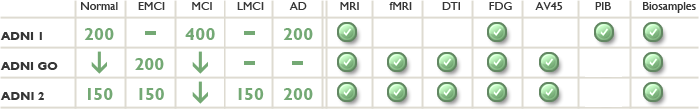
\includegraphics[width=\textwidth]{study-design.png}
  \caption{\label{fig:design}ADNI study design}
\end{figure}

The table below summarizes the numbers for the \textbf{ADNI1} cohort
only, for the MRI and PET modalities.

\begin{tabular}[H]{c | c | c | c | c | c}
  & NL & \multicolumn{3}{|c|}{MCI} & AD\\
\hline
& & MCI-c & MCI-nc & MCI-rev &\\
\hline
FDG-PET & 102 & 94 & 96 & 13 & 97\\
MRI(clean) & 180 & 133 & 132 & 10 & 123\\
MRI(complete) & 229 & 196 & 183 & 18 & 192\\
FDG+MRI(clean) & 79 & 66 & 68 & 9 & 62\\
FDG+MRI(complete) & 102 & 94 & 96 & 13 & 97\\
\end{tabular}

\section{SVMs on classification task}
\label{sec:svm}

All of the following classification results are based only on features
evaluated for the patients at \textbf{baseline}.

\subsection{MCI-c vs MCI-nc}
\label{sec:mci-c-nc}

MCI-c is the group that goes on to convert to AD in any of their
subsequent follow-ups. The maximum span for this can be upto 4 years.

MCI-nc is the group that stays stable in all subsequent
follow-ups. 

Note that the patients in both groups \textbf{do not} have the same
follow-ups - it is highly possible some patients in MCI-nc have much
fewer follow-ups that MCI-c patients and have just not been detected
as converters.

\subsubsection{Hyper-parameter search}
\label{sec:mci-c-nc-hyper}

\begin{figure}[H]
  \centering
  \begin{subfigure}[h]{0.49\textwidth}
    \includegraphics[width=\textwidth]{mci-c-nc/MRI:hyper-auroc.png}
    \caption{Optimizing for ROC-AUC}  
  \end{subfigure}
  \begin{subfigure}[h]{0.49\textwidth}
    \includegraphics[width=\textwidth]{mci-c-nc/MRI:hyper-acc.png}
    \caption{Optimizing for accuracy}  
  \end{subfigure}
  \caption{Hyper-parameter search using MRI-based features}
\end{figure}

\begin{figure}[H]
  \centering
  \begin{subfigure}[h]{0.49\textwidth}
    \includegraphics[width=\textwidth]{mci-c-nc/PET:hyper-auroc.png}
    \caption{Optimizing for ROC-AUC}  
  \end{subfigure}
  \begin{subfigure}[h]{0.49\textwidth}
    \includegraphics[width=\textwidth]{mci-c-nc/PET:hyper-acc.png}
    \caption{Optimizing for accuracy}  
  \end{subfigure}
  \caption{Hyper-parameter search using PET-based features}
\end{figure}

\begin{figure}[H]
  \centering
  \begin{subfigure}[h]{0.49\textwidth}
    \includegraphics[width=\textwidth]{mci-c-nc/CAT:hyper-auroc.png}
    \caption{Optimizing for ROC-AUC}  
  \end{subfigure}
  \begin{subfigure}[h]{0.49\textwidth}
    \includegraphics[width=\textwidth]{mci-c-nc/CAT:hyper-acc.png}
    \caption{Optimizing for accuracy}  
  \end{subfigure}
  \caption{Hyper-parameter search using conCATenated features}
\end{figure}

\subsubsection{Classification results}
\label{sec:mci-c-nc-res}

\begin{figure}[H]
  \centering
  \begin{subfigure}[h]{0.49\textwidth}
    \includegraphics[width=\textwidth]{mci-c-nc/MRI:acc.png}
    \caption{Classification accuracy}  
  \end{subfigure}
  \begin{subfigure}[h]{0.49\textwidth}
    \includegraphics[width=\textwidth]{mci-c-nc/MRI:roc.png}
    \caption{ROC curves}  
  \end{subfigure}
  \caption{Classification results using MRI-based features}
\end{figure}

\begin{figure}[H]
  \centering
  \begin{subfigure}[h]{0.49\textwidth}
    \includegraphics[width=\textwidth]{mci-c-nc/PET:acc.png}
    \caption{Classification accuracy}  
  \end{subfigure}
  \begin{subfigure}[h]{0.49\textwidth}
    \includegraphics[width=\textwidth]{mci-c-nc/PET:roc.png}
    \caption{ROC curves}  
  \end{subfigure}
  \caption{Classification results using PET-based features}
\end{figure}

\begin{figure}[H]
  \centering
  \begin{subfigure}[h]{0.49\textwidth}
    \includegraphics[width=\textwidth]{mci-c-nc/CAT:acc.png}
    \caption{Classification accuracy}  
  \end{subfigure}
  \begin{subfigure}[h]{0.49\textwidth}
    \includegraphics[width=\textwidth]{mci-c-nc/CAT:roc.png}
    \caption{ROC curves}  
  \end{subfigure}
  \caption{Classification results using CAT-based features}
\end{figure}

\subsubsection{State of the Art}
\label{sec:mci-c-nc-soa}

Zhang multi-modal multi-kernel:

MRI: $62\%$\\
PET: $63.9\%$\\
CSF: $51.8\%$\\
CONCAT(all three): $65.4\%$\\
Proposed: $73.9\%$\\

\subsection{NL vs MCI}
\label{sec:nl-mci}

\subsubsection{Hyper-parameter search}
\label{sec:nl-mci-hyper}

\begin{figure}[H]
  \centering
  \begin{subfigure}[h]{0.49\textwidth}
    \includegraphics[width=\textwidth]{nl-mci/MRI:hyper-auroc.png}
    \caption{Optimizing for ROC-AUC}  
  \end{subfigure}
  \begin{subfigure}[h]{0.49\textwidth}
    \includegraphics[width=\textwidth]{nl-mci/MRI:hyper-acc.png}
    \caption{Optimizing for accuracy}  
  \end{subfigure}
  \caption{Hyper-parameter search using MRI-based features}
\end{figure}

\begin{figure}[H]
  \centering
  \begin{subfigure}[h]{0.49\textwidth}
    \includegraphics[width=\textwidth]{nl-mci/PET:hyper-auroc.png}
    \caption{Optimizing for ROC-AUC}  
  \end{subfigure}
  \begin{subfigure}[h]{0.49\textwidth}
    \includegraphics[width=\textwidth]{nl-mci/PET:hyper-acc.png}
    \caption{Optimizing for accuracy}  
  \end{subfigure}
  \caption{Hyper-parameter search using PET-based features}
\end{figure}

\begin{figure}[H]
  \centering
  \begin{subfigure}[h]{0.49\textwidth}
    \includegraphics[width=\textwidth]{nl-mci/CAT:hyper-auroc.png}
    \caption{Optimizing for ROC-AUC}  
  \end{subfigure}
  \begin{subfigure}[h]{0.49\textwidth}
    \includegraphics[width=\textwidth]{nl-mci/CAT:hyper-acc.png}
    \caption{Optimizing for accuracy}  
  \end{subfigure}
  \caption{Hyper-parameter search using conCATenated features}
\end{figure}

\subsubsection{Classification results}
\label{sec:nl-mci-res}

\begin{figure}[H]
  \centering
  \begin{subfigure}[h]{0.49\textwidth}
    \includegraphics[width=\textwidth]{nl-mci/MRI:acc.png}
    \caption{Classification accuracy}  
  \end{subfigure}
  \begin{subfigure}[h]{0.49\textwidth}
    \includegraphics[width=\textwidth]{nl-mci/MRI:roc.png}
    \caption{ROC curves}  
  \end{subfigure}
  \caption{Classification results using MRI-based features}
\end{figure}

\begin{figure}[H]
  \centering
  \begin{subfigure}[h]{0.49\textwidth}
    \includegraphics[width=\textwidth]{nl-mci/PET:acc.png}
    \caption{Classification accuracy}  
  \end{subfigure}
  \begin{subfigure}[h]{0.49\textwidth}
    \includegraphics[width=\textwidth]{nl-mci/PET:roc.png}
    \caption{ROC curves}  
  \end{subfigure}
  \caption{Classification results using PET-based features}
\end{figure}

\begin{figure}[H]
  \centering
  \begin{subfigure}[h]{0.49\textwidth}
    \includegraphics[width=\textwidth]{nl-mci/CAT:acc.png}
    \caption{Classification accuracy}  
  \end{subfigure}
  \begin{subfigure}[h]{0.49\textwidth}
    \includegraphics[width=\textwidth]{nl-mci/CAT:roc.png}
    \caption{ROC curves}  
  \end{subfigure}
  \caption{Classification results using CAT-based features}
\end{figure}

\subsubsection{State of the Art}
\label{sec:nl-mci-soa}

Zhang multi-modal:

MRI: $72\%$\\
PET: $71.6\%$\\
CSF: $71.4\%$\\
ALL: $76.4\%$\\

\subsection{NL vs AD}
\label{sec:nl-ad}

\subsubsection{Hyper-parameter search}
\label{sec:nl-ad-hyper}

\begin{figure}[H]
  \centering
  \begin{subfigure}[h]{0.49\textwidth}
    \includegraphics[width=\textwidth]{nl-ad/MRI:hyper-auroc.png}
    \caption{Optimizing for ROC-AUC}  
  \end{subfigure}
  \begin{subfigure}[h]{0.49\textwidth}
    \includegraphics[width=\textwidth]{nl-ad/MRI:hyper-acc.png}
    \caption{Optimizing for accuracy}  
  \end{subfigure}
  \caption{Hyper-parameter search using MRI-based features}
\end{figure}

\begin{figure}[H]
  \centering
  \begin{subfigure}[h]{0.49\textwidth}
    \includegraphics[width=\textwidth]{nl-ad/PET:hyper-auroc.png}
    \caption{Optimizing for ROC-AUC}  
  \end{subfigure}
  \begin{subfigure}[h]{0.49\textwidth}
    \includegraphics[width=\textwidth]{nl-ad/PET:hyper-acc.png}
    \caption{Optimizing for accuracy}  
  \end{subfigure}
  \caption{Hyper-parameter search using PET-based features}
\end{figure}

\begin{figure}[H]
  \centering
  \begin{subfigure}[h]{0.49\textwidth}
    \includegraphics[width=\textwidth]{nl-ad/CAT:hyper-auroc.png}
    \caption{Optimizing for ROC-AUC}  
  \end{subfigure}
  \begin{subfigure}[h]{0.49\textwidth}
    \includegraphics[width=\textwidth]{nl-ad/CAT:hyper-acc.png}
    \caption{Optimizing for accuracy}  
  \end{subfigure}
  \caption{Hyper-parameter search using conCATenated features}
\end{figure}

\subsubsection{Classification results}
\label{sec:nl-ad-res}

\begin{figure}[H]
  \centering
  \begin{subfigure}[h]{0.49\textwidth}
    \includegraphics[width=\textwidth]{nl-ad/MRI:acc.png}
    \caption{Classification accuracy}  
  \end{subfigure}
  \begin{subfigure}[h]{0.49\textwidth}
    \includegraphics[width=\textwidth]{nl-ad/MRI:roc.png}
    \caption{ROC curves}  
  \end{subfigure}
  \caption{Classification results using MRI-based features}
\end{figure}

\begin{figure}[H]
  \centering
  \begin{subfigure}[h]{0.49\textwidth}
    \includegraphics[width=\textwidth]{nl-ad/PET:acc.png}
    \caption{Classification accuracy}  
  \end{subfigure}
  \begin{subfigure}[h]{0.49\textwidth}
    \includegraphics[width=\textwidth]{nl-ad/PET:roc.png}
    \caption{ROC curves}  
  \end{subfigure}
  \caption{Classification results using PET-based features}
\end{figure}

\begin{figure}[H]
  \centering
  \begin{subfigure}[h]{0.49\textwidth}
    \includegraphics[width=\textwidth]{nl-ad/CAT:acc.png}
    \caption{Classification accuracy}  
  \end{subfigure}
  \begin{subfigure}[h]{0.49\textwidth}
    \includegraphics[width=\textwidth]{nl-ad/CAT:roc.png}
    \caption{ROC curves}  
  \end{subfigure}
  \caption{Classification results using CAT-based features}
\end{figure}

\subsubsection{State of the Art}
\label{sec:nl-ad-soa}

Zhang multi-modal kernel:

MRI: $86.2\%$\\
PET: $86.5\%$\\
CSF: $82.1\%$\\
ALL: $93.2\%$\\

\subsection{MCI vs AD}
\label{sec:mci-ad}

\subsubsection{Hyper-parameter search}
\label{sec:mci-ad-hyper}

\begin{figure}[H]
  \centering
  \begin{subfigure}[h]{0.49\textwidth}
    \includegraphics[width=\textwidth]{mci-ad/MRI:hyper-auroc.png}
    \caption{Optimizing for ROC-AUC}  
  \end{subfigure}
  \begin{subfigure}[h]{0.49\textwidth}
    \includegraphics[width=\textwidth]{mci-ad/MRI:hyper-acc.png}
    \caption{Optimizing for accuracy}  
  \end{subfigure}
  \caption{Hyper-parameter search using MRI-based features}
\end{figure}

\begin{figure}[H]
  \centering
  \begin{subfigure}[h]{0.49\textwidth}
    \includegraphics[width=\textwidth]{mci-ad/PET:hyper-auroc.png}
    \caption{Optimizing for ROC-AUC}  
  \end{subfigure}
  \begin{subfigure}[h]{0.49\textwidth}
    \includegraphics[width=\textwidth]{mci-ad/PET:hyper-acc.png}
    \caption{Optimizing for accuracy}  
  \end{subfigure}
  \caption{Hyper-parameter search using PET-based features}
\end{figure}

\begin{figure}[H]
  \centering
  \begin{subfigure}[h]{0.49\textwidth}
    \includegraphics[width=\textwidth]{mci-ad/CAT:hyper-auroc.png}
    \caption{Optimizing for ROC-AUC}  
  \end{subfigure}
  \begin{subfigure}[h]{0.49\textwidth}
    \includegraphics[width=\textwidth]{mci-ad/CAT:hyper-acc.png}
    \caption{Optimizing for accuracy}  
  \end{subfigure}
  \caption{Hyper-parameter search using conCATenated features}
\end{figure}

\subsubsection{Classification results}
\label{sec:mci-ad-res}

\begin{figure}[H]
  \centering
  \begin{subfigure}[h]{0.49\textwidth}
    \includegraphics[width=\textwidth]{mci-ad/MRI:acc.png}
    \caption{Classification accuracy}  
  \end{subfigure}
  \begin{subfigure}[h]{0.49\textwidth}
    \includegraphics[width=\textwidth]{mci-ad/MRI:roc.png}
    \caption{ROC curves}  
  \end{subfigure}
  \caption{Classification results using MRI-based features}
\end{figure}

\begin{figure}[H]
  \centering
  \begin{subfigure}[h]{0.49\textwidth}
    \includegraphics[width=\textwidth]{mci-ad/PET:acc.png}
    \caption{Classification accuracy}  
  \end{subfigure}
  \begin{subfigure}[h]{0.49\textwidth}
    \includegraphics[width=\textwidth]{mci-ad/PET:roc.png}
    \caption{ROC curves}  
  \end{subfigure}
  \caption{Classification results using PET-based features}
\end{figure}

\begin{figure}[H]
  \centering
  \begin{subfigure}[h]{0.49\textwidth}
    \includegraphics[width=\textwidth]{mci-ad/CAT:acc.png}
    \caption{Classification accuracy}  
  \end{subfigure}
  \begin{subfigure}[h]{0.49\textwidth}
    \includegraphics[width=\textwidth]{mci-ad/CAT:roc.png}
    \caption{ROC curves}  
  \end{subfigure}
  \caption{Classification results using CAT-based features}
\end{figure}

\subsubsection{State of the Art}
\label{sec:mci-ad-soa}

\end{document}